\begin{subsection}{Diagrama de objectivos}
La figura \ref{fig:diagrama_objetivos} puede verse el diagrama de objetivos propuesto, que describe todos los objetivos del problema de las ciclovías.

\begin{figure}[H]
        \centering
        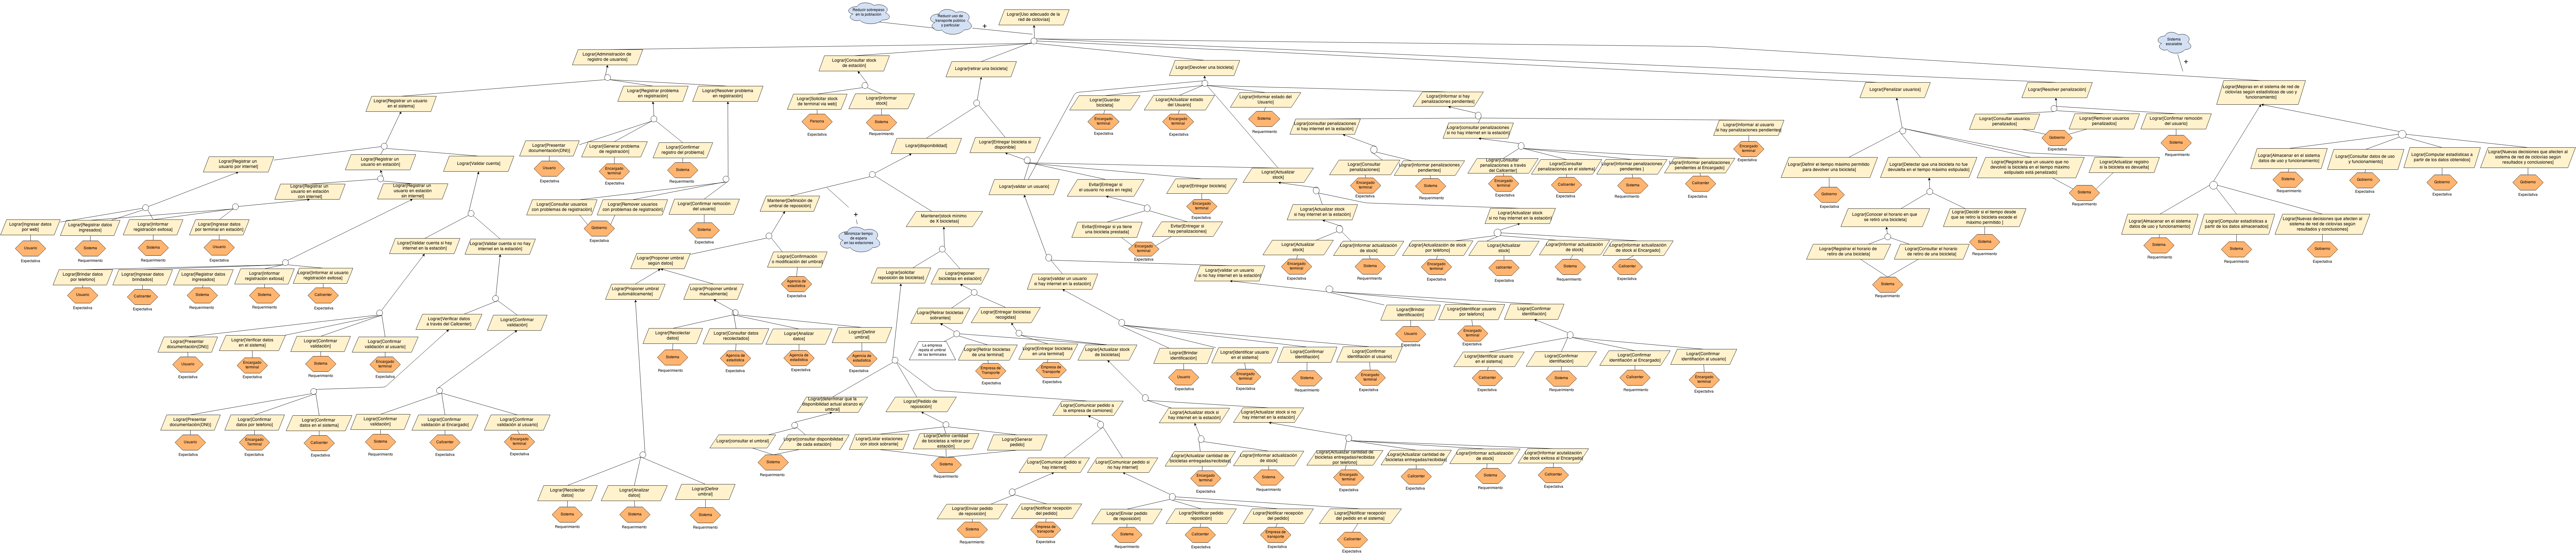
\includegraphics[angle=90,width=\textwidth,height=\textheight,keepaspectratio]{imagenes/diagrama_de_objetivos.png}
        \caption{diagrama de objetivos}
        \label{fig:diagrama_objetivos}
\end{figure}

\begin{figure}[H]
        \centering
        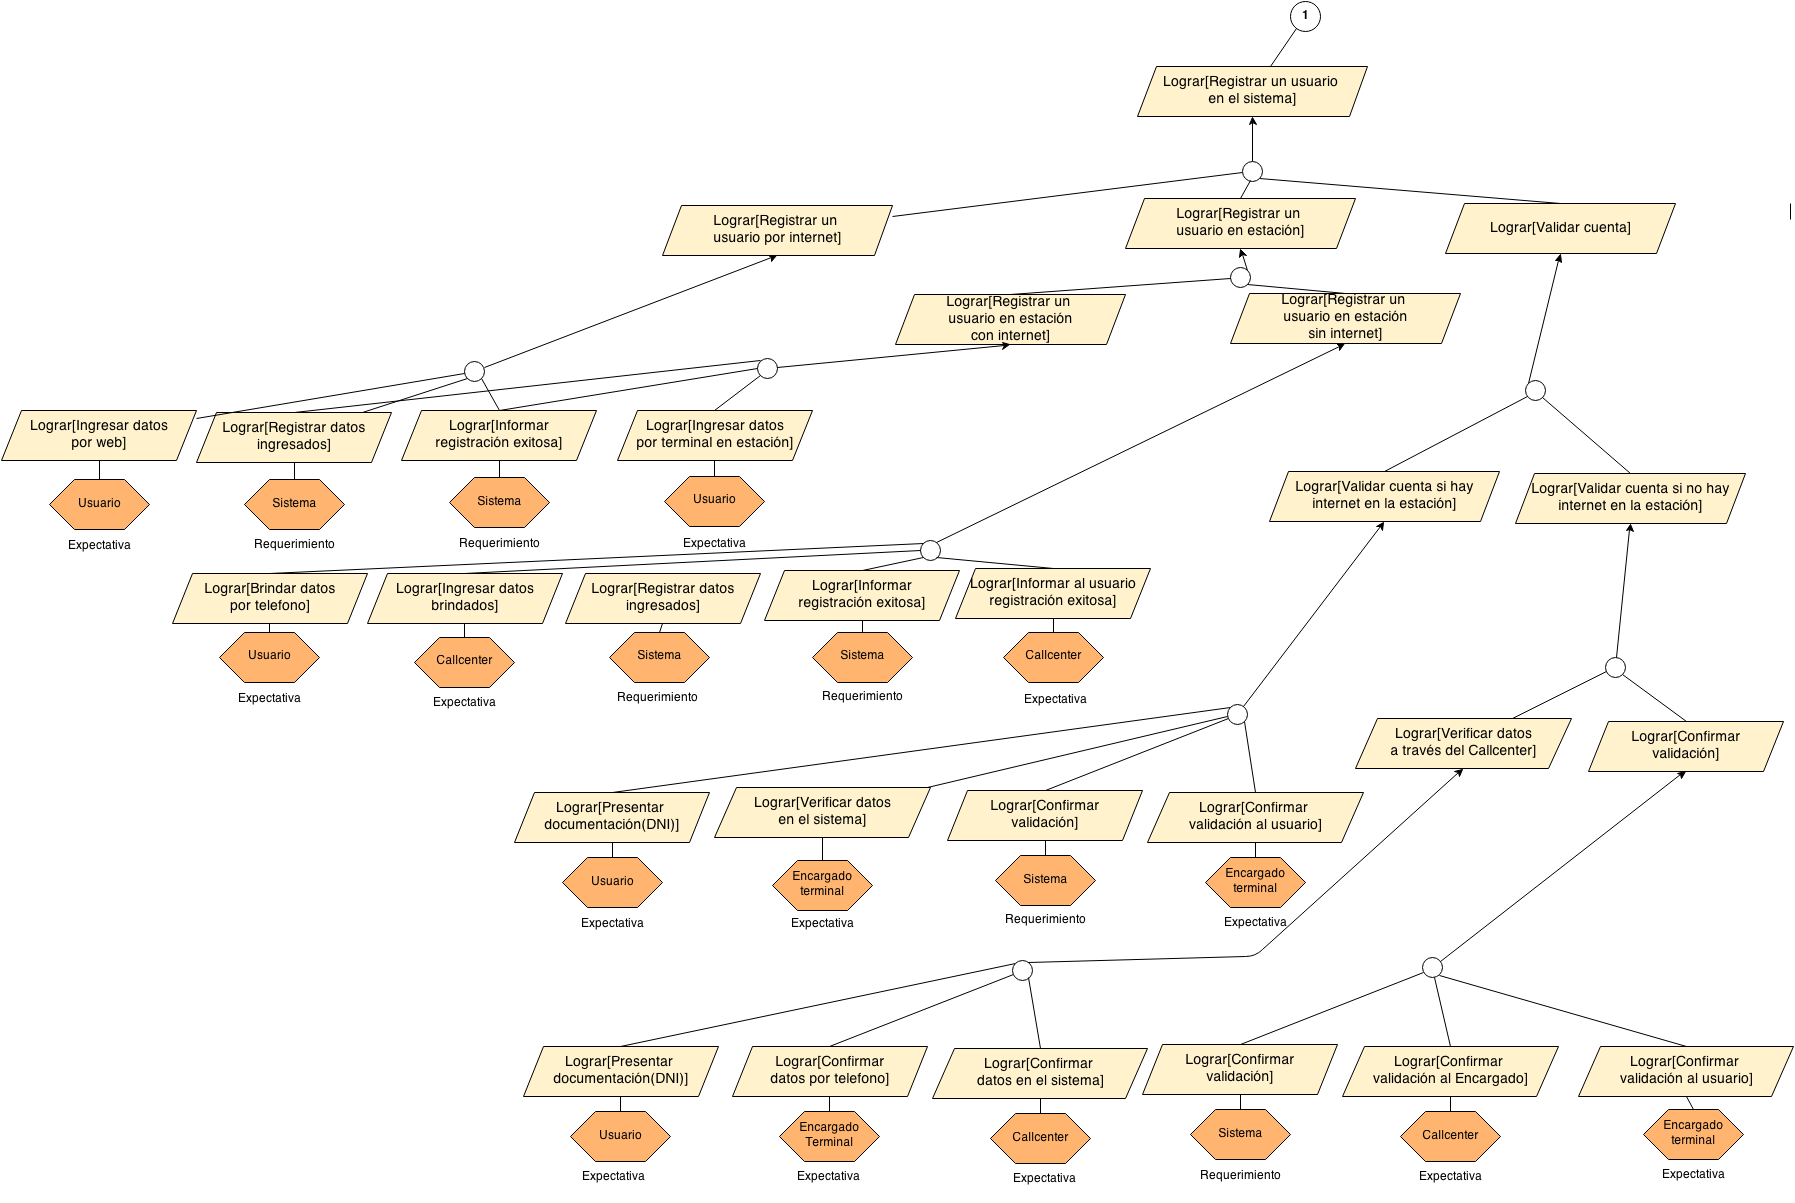
\includegraphics[angle=90,width=\textwidth,height=\textheight,keepaspectratio]{imagenes/do_1.png}
        \caption{diagrama de objetivos - 1}
        \label{fig:diagrama_objetivos_1}
\end{figure}

\begin{figure}[H]
        \centering
        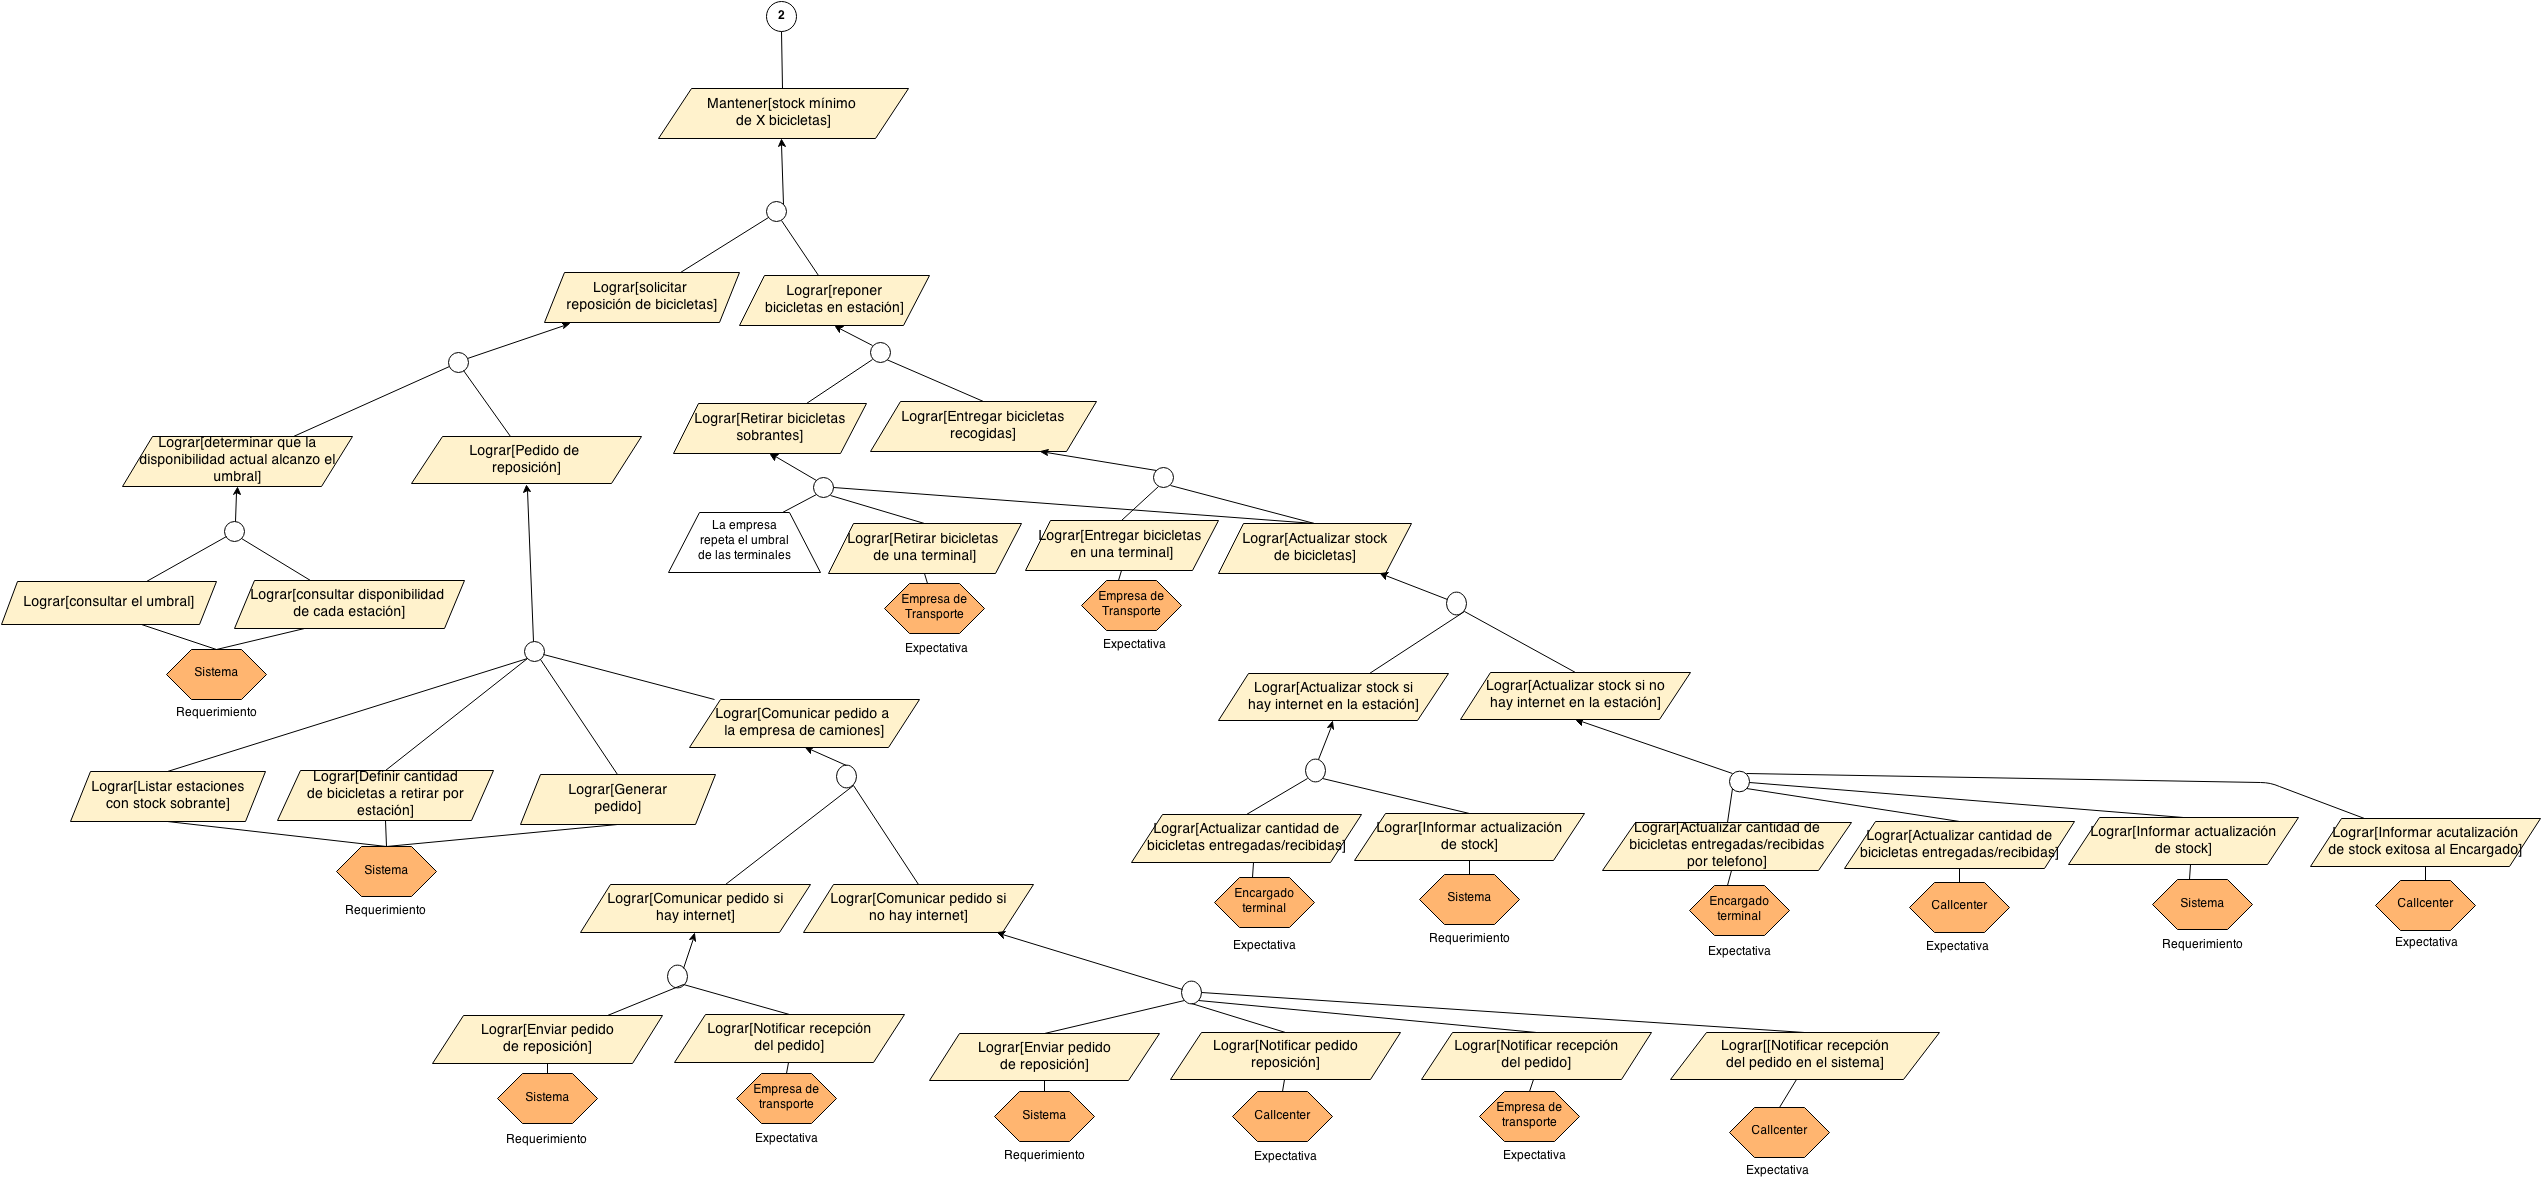
\includegraphics[angle=90,width=\textwidth,height=\textheight,keepaspectratio]{imagenes/do_2.png}
        \caption{diagrama de objetivos - 2}
        \label{fig:diagrama_objetivos_2}
\end{figure}


\begin{figure}[H]
        \centering
        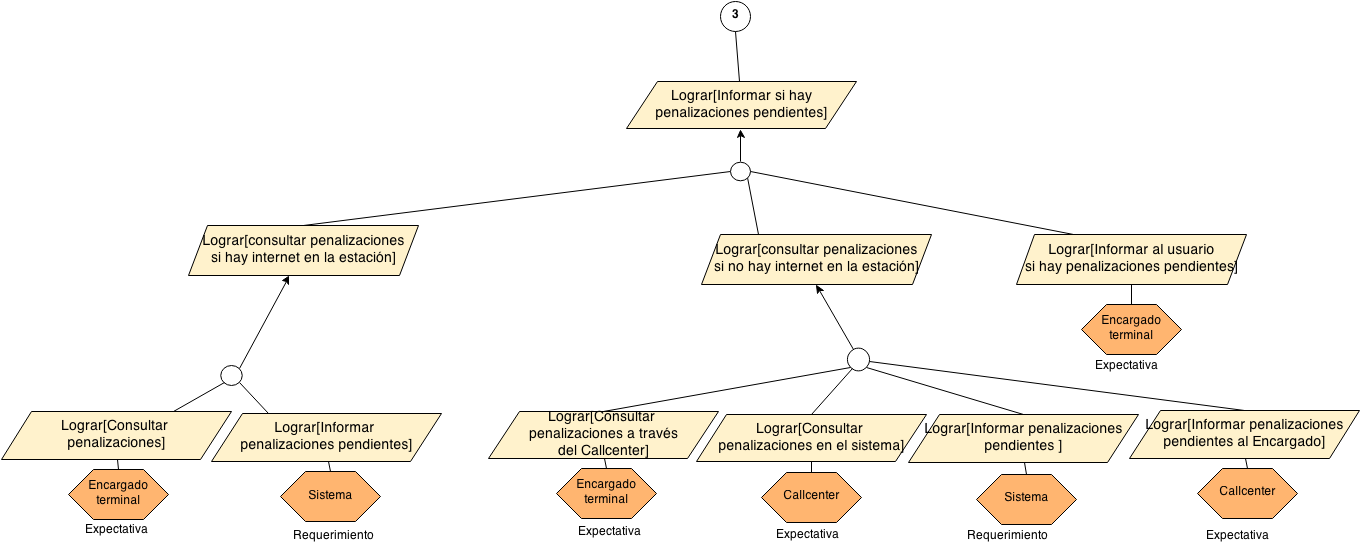
\includegraphics[angle=90,width=\textwidth,height=\textheight,keepaspectratio]{imagenes/do_3.png}
        \caption{diagrama de objetivos - 3}
        \label{fig:diagrama_objetivos_3}
\end{figure}

\begin{figure}[H]
        \centering
        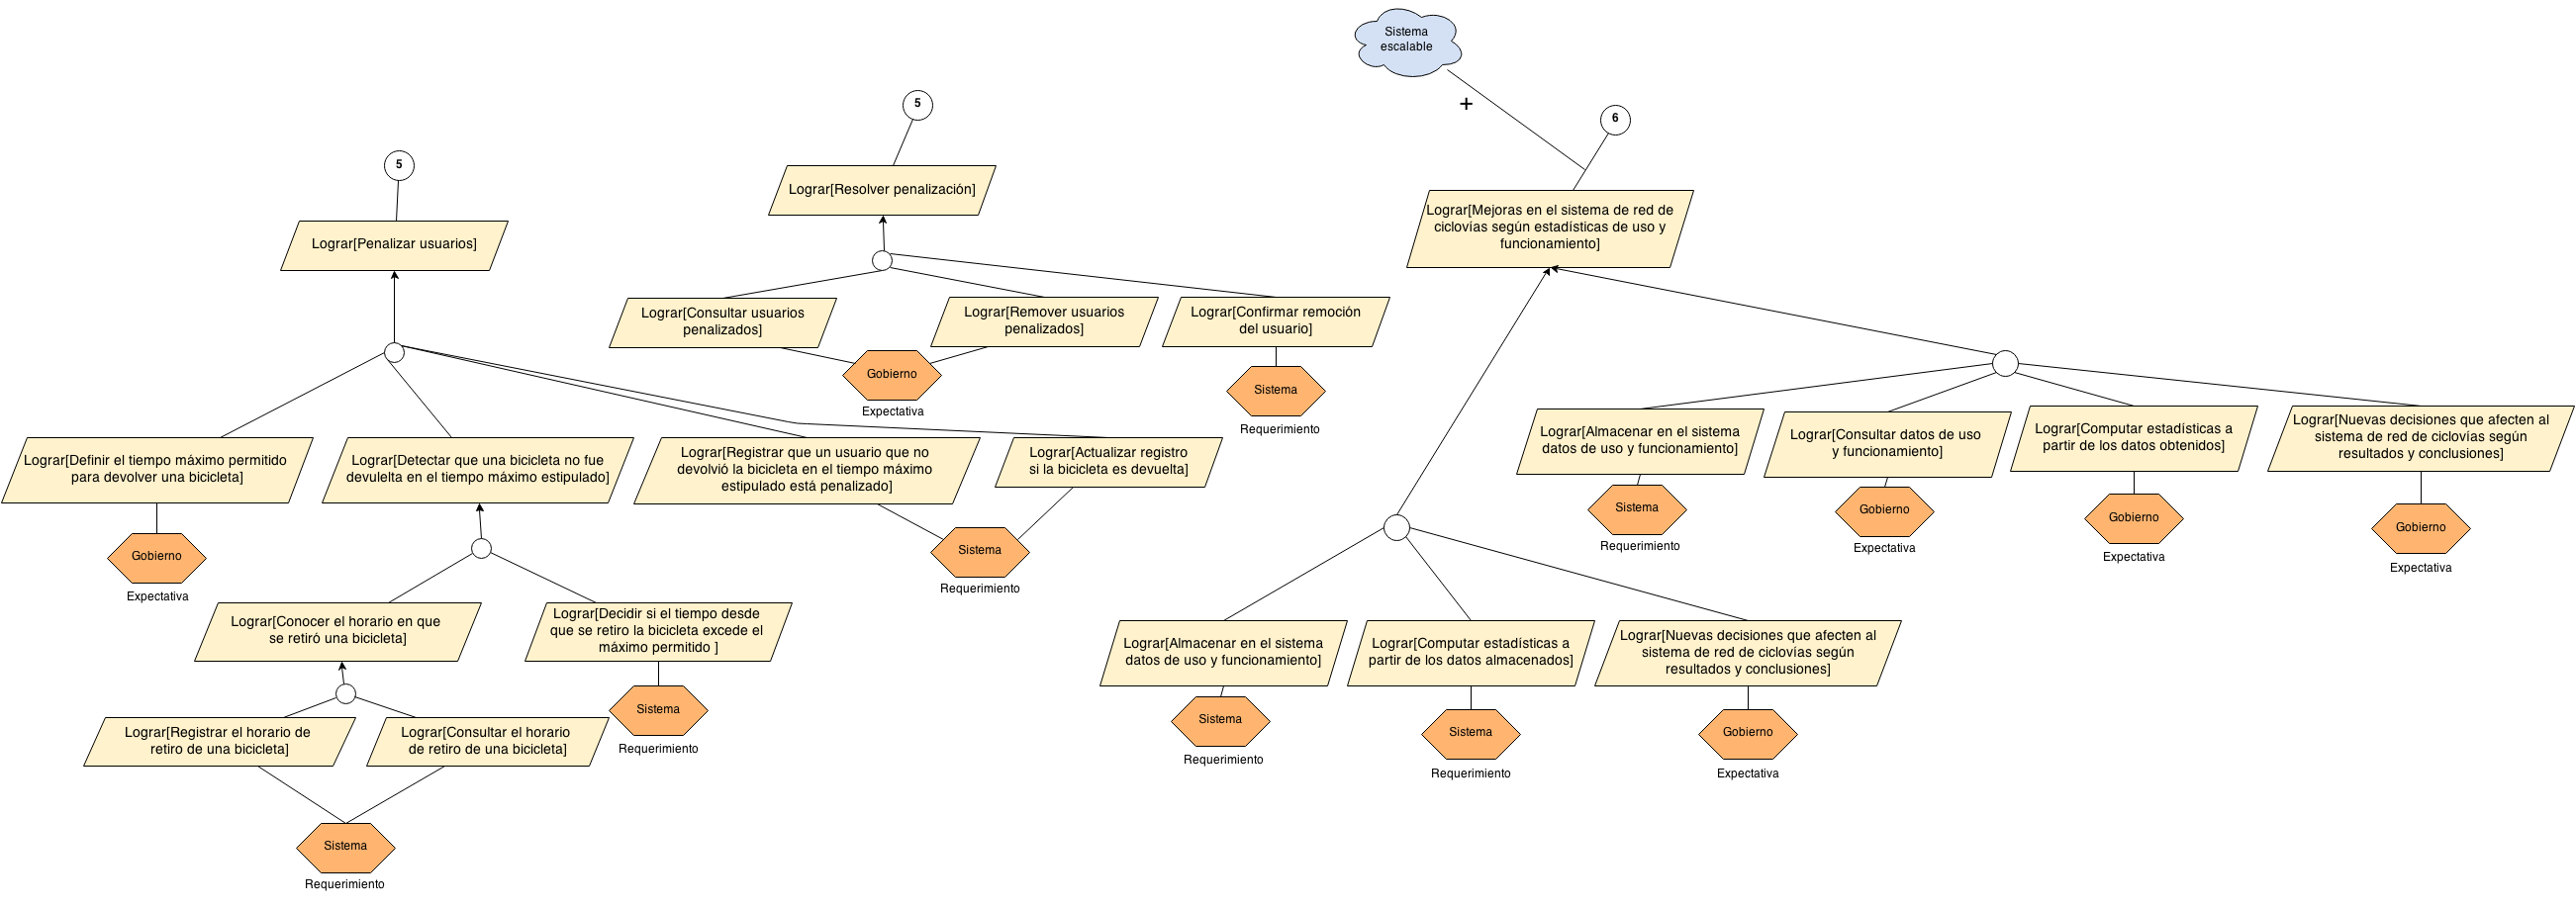
\includegraphics[angle=90,width=\textwidth,height=\textheight,keepaspectratio]{imagenes/do_4-5-6.png}
        \caption{diagrama de objetivos - 4 5 6}
        \label{fig:diagrama_objetivos_4_5_6}
\end{figure}
%\begin{figure}[H]
%	
%	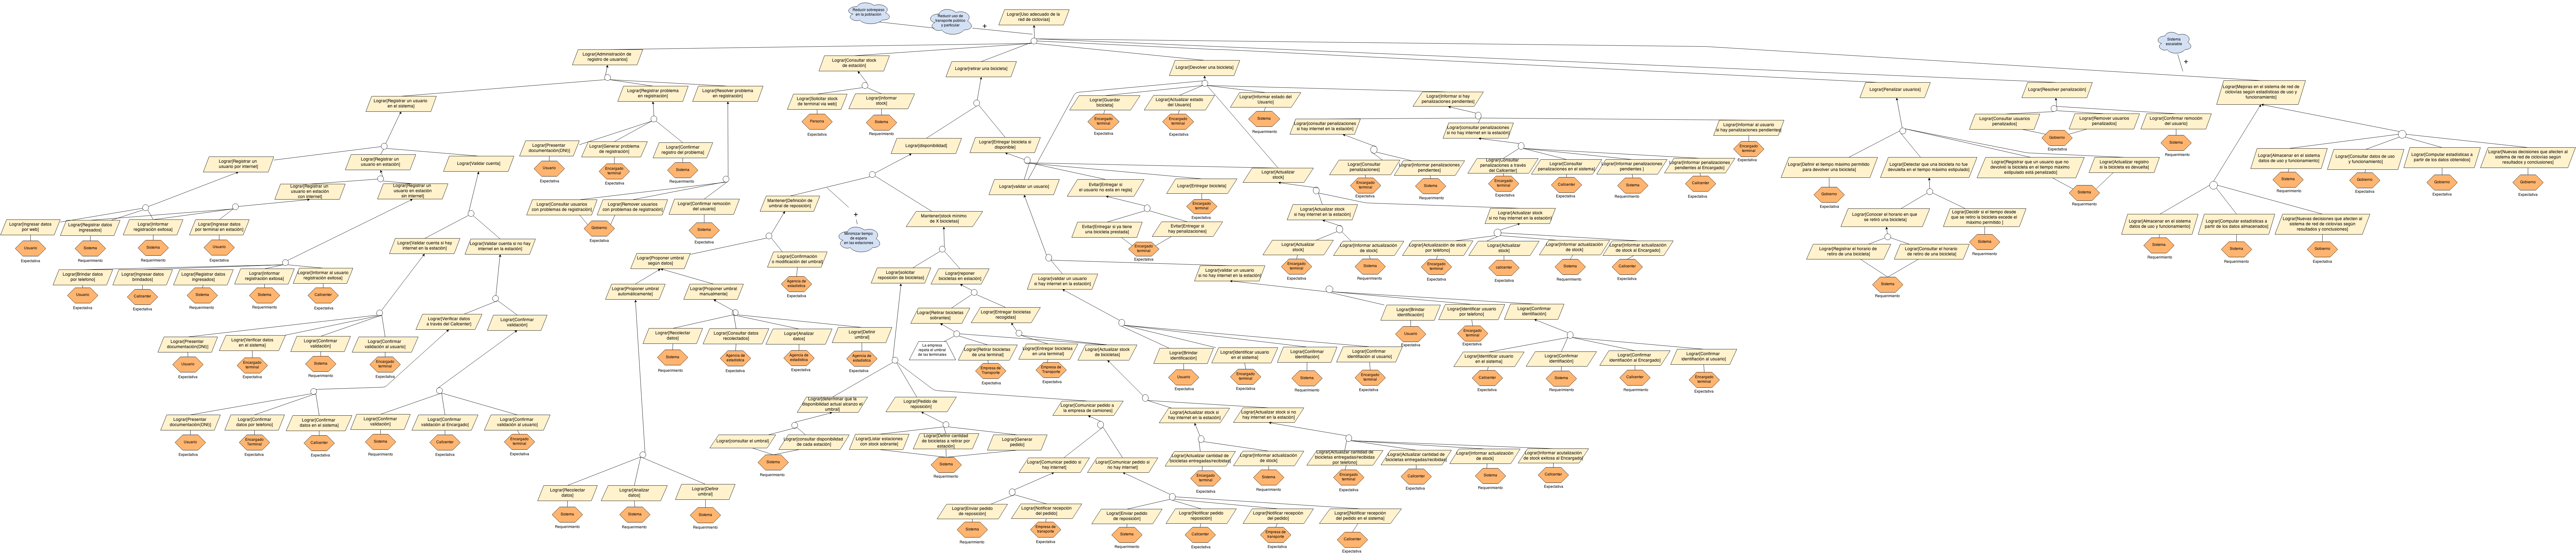
\includegraphics[scale=0.47]{imagenes/diagrama_de_objetivos.png}
%	\caption{diagrama de contexto}
%	\label{fig:diagrama_objetivos}
%
%\end{figure}

\end{subsection}

%\begin{subsection}{Análisis de objetivos}

%\end{subsection}